\chapter{Introducere \^{\i}n reţelele definite prin software\label{ch:introducere_sdn}}

\graphicspath{ {cap-introducere_in_sdn/figures/} }

În zilele noastre, reţelele de comunicaţii au devenit complexe și greu de administrat și configurat. De asemenea, numărul dispozitivelor mobile a crescut considerabil, alături de conţinutul pe care acestea îl accesează. Aceste lucruri au dus la evidenţierea limitărilor pe care reţelele tradiţionale le presupun. Chiar dacă nu toate ideile ce stau la baza ei sunt noi, datorită unui context favorabil, acestea, împreună cu alte noi idei, au dus la apariţia paradigmei \gls{sdn} în industria reţelisticii.

Această nouă tehnologie nu a ajuns încă la maturitate și la adoptarea pe scară largă, în toate aspectele reţelelor, însă eforturile considerabile care se fac în activităţile de standardizare și crearea de ecosisteme \gls{sdn} vor duce la această adoptare. După cum este evidenţiat și în~\cite{nadeau2013sdn}, se tinde către crearea unor reţele care pot fi programate prin software, crescând astfel flexibilitatea și agilitatea lor.

\section{Istoria și evoluția SDN}

\subsection{Istoria SDN}

Reţelele definite prin software îşi au originile în activitatea și ideile din cadrul proiectului OpenFlow, început la universitatea Stanford, în jurul anului 2009. Multe dintre conceptele și ideile folosite în \gls{sdn} au evoluat însă în ultimii 25 de ani și acum îşi găsesc locul în această nouă paradigmă, care îşi propune să schimbe modul în care reţelele sunt proiectate și administrate.

\gls{sdn} reprezintă o arhitectură nouă de reţea, în care starea de dirijare a planului de date este administrată de un plan de control distant, decuplat de cel de date. Reţelele definite prin software reprezintă o arhitectură de rețea ce se bazează pe următoarele 4 concepte, conform~\cite{kreutz2015software}:
\begin{enumerate}
	\item Decuplarea planurilor de date și de control;
	\item Deciziile de dirijare se bazează pe fluxuri de date, nu pe adresa destinaţie;
	\item Logica de control se mută într-o entitate externă, un echipament de control \gls{sdn} (care are un sistem de operare de reţea);
	\item Reţeaua este programabilă prin aplicaţii software care rulează peste sistemul de operare de reţea și care interacţionează cu echipamentele din planul de date.
\end{enumerate}

Reţelele definite prin programe software au apărut în scopul de a oferi posibilitatea inovaţiei în cadrul administrării reţelelor și pentru a uşura introducerea de noi servicii. Aceste nevoi nu sunt însă noi, ele mai fiind studiate și în trecut, însă abia acum, prin \gls{sdn}, pot fi satisfăcute într-un mod viabil, fără a implica schimbări majore în infrastructura reţelelor deja existente.

Istoria \gls{sdn} poate fi împărţită în trei etape, fiecare influenţând această nouă paradigmă prin conceptele propuse, aşa cum este evidenţiat în~\cite{feamster2014road}:
\begin{enumerate}
	\item Reţelele active, care au introdus funcţiile programabile în reţea, sporind gradul de inovaţie (mijlocul anilor 1990 – începutul anilor 2000);
	\item Separarea planurilor de date și de control, care a condus la dezvoltarea de interfeţe deschise între planurile de date și de control (aproximativ 2001 – 2007);
	\item Dezvoltarea protocolului OpenFlow și a sistemelor de operare de reţea, care reprezintă prima adoptare pe scară largă a unei interfeţe deschise, făcând separarea planurilor de control și de date extensibilă și practică.
\end{enumerate}

\subsubsection{Rețelele active}

Reţelele active reprezintă reţele în care comutatoarele pot efectua anumite calcule sau operaţii asupra pachetelor de date. Reţelele tradiţionale nu pot fi considerate programabile. Reţelele active au reprezentat o schimbare de concept radicală asupra controlului unei reţele, propunând o interfaţă de programare care să expună resurse în noduri individuale de reţea și să susţină construirea de funcţionalităţi specifice, care să fie aplicate unui subset de pachete care tranzitează acel nod.

Motivul principal pentru care reţelele active au apărut a fost cel de accelerare a inovației. La momentul respectiv, introducerea unui nou concept, serviciu sau tehnologie, într-o reţea de mari dimensiuni, cum ar fi Internet-ul, putea dura până la zece ani, de la faza de prototip până la implementare. Se dorea ca nodurile active din reţea să permită ruterelor/comutatoarelor să descarce și să implementeze servicii noi în infrastructura deja existentă. În acelaşi timp, aceste noduri active ar fi putut coexista fără probleme în aceeaşi reţea cu vechile dispozitive.

Au existat două tipuri de abordări în cadrul reţelelor active, în funcţie de modelul ales pentru programarea rețelei:
\begin{itemize}
\item \textit{Modelul încapsulat} – unde codul care trebuia executat în cadrul nodurilor active era transportat în bandă, în pachetele de date; fiecare pachet de date conţinea cod care trebuia rulat;
\item \textit{Modelul comutatoarelor programabile} – codul care trebuia executat în cadrul nodurilor active era stabilit prin mecanisme din afara benzii. Execuţia programelor era determinată de antetul pachetului.
\end{itemize}

Rețelele active nu au ajuns niciodată să fie implementate pe scară largă, din mai multe cauze: momentul de timp la care au apărut acestea nu a fost potrivit; la acel moment nu aveau o aplicabilitate clară, deoarece nu apăruseră încă centrele de date sau infrastructurile de tip cloud; implementarea reţelelor active avea nevoie și de suport hardware, care nu era tocmai ieftin, ceea ce a constituit încă un dezavantaj.

Chiar dacă rețelele active nu au ajuns să fie implementate pe scară largă, câteva idei au fost preluate în cadrul rețelelor definite prin programe software:
\begin{itemize}
\item \textbf{Funcţii programabile în rețea, care să faciliteze inovaţia.} În motivaţia introducerii rețelelor definite prin software se acuză dificultatea inovației în rețelele de producţie. Rețelele active foloseau programarea planului de date, în timp ce în \gls{sdn} se programează atât planul de control cât și cel de date.
\item \textbf{Virtualizarea rețelei și capacitatea de a demultiplexa programe soft pe baza antetului pachetelor.} Rețelele active au dezvoltat un cadru arhitectural care să permită funcționarea unei astfel de platforme, având drept componente de bază un sistem de operare comun (al nodurilor), un set de medii de execuţie și un set de aplicații active, care oferă de fapt un serviciu capăt-la-capăt.
\item \textbf{Atenţia la aparatele de rețea și la felul în care funcţiile acestora sunt compuse.} În cercetarea din cadrul rețelelor active se vorbea despre nevoia unificării gamei largi de funcţii oferite de aparatele de rețea într-un cadru programabil sigur.
\end{itemize}

\subsubsection{Separarea planurilor de date și de control}

Rețelele, încă de la început, au avut planurile de date și de control integrate. Acest lucru a dus la câteva dezavantaje: îngreunarea sarcinilor de administrare a rețelei, de depanare a configurării rețelei sau de controlul/prezicerea comportamentului de dirijare.

Primele inițiative de separare a planurilor de control și de date datează din anii 1980. La acel moment, cei de la AT\&T propuneau renunţarea la semnalizarea în bandă și introducerea unui Punct de Control al Rețelei - \gls{ncp}, realizând astfel separarea planurilor de control și de date. Această modificare a înlesnit accelerarea inovației în rețea, prin posibilitatea de introducere rapidă de noi servicii și a furnizat noi metode de a îmbunătăţi eficienţa, prin introducerea unei vederi de ansamblu asupra rețelei oferită de punctul de control al rețelei. Există și inițiative mai recente care și-au propus separarea planurilor de control și de date, cum ar fi ETHANE~\cite{casado2007ethane}, NOX~\cite{gude2008nox}, OpenFlow~\cite{mckeown2008openflow}. Acestea au ca avantaj faptul că nu au nevoie de modificări substanţiale în echipamentele de dirijare, ceea ce înseamnă că pot fi adoptate mai ușor de către industria rețelelor.

Ideile preluate în rețelele definite prin programe software din cercetarea care propunea separarea planurilor de control și de date sunt următoarele:
\begin{itemize}
	\item \textbf{Control logic centralizat care folosește o interfață deschisă către planul de date.} O interfață deschisă către planul de date, care să permită inovația în aplicațiile software din planul de control a fost propusă de activitățile de cercetare din cadrul ForCES~\cite{haleplidis2015network}. Însă, această interfață nu a fost adoptată de marile companii furnizoare de echipamente de rețea, astfel că aceasta nu a fost implementată pe scară largă.
	\item \textbf{Administrarea stărilor distribuite.} Controlul logic centralizat al rețelei a atras alte provocări, cum ar fi administrarea stărilor distribuite. Un echipament de control logic centralizat trebuie reprodus pentru a face față defectării acestuia. Însă această reproducere poate duce la stări de inconsistență între copiile echipamentului de control. Aceste probleme apar și în cadrul \gls{sdn}, în contextul echipamentelor de control distribuite.
\end{itemize}

\subsubsection{Protocolul OpenFlow și sistemele de operare de rețea}

Înainte de apariţia protocolului OpenFlow, ideile care stăteau la baza rețelelor definite prin programe software aveau parte de o contradicţie între viziunea unor rețele complet programabile și pragmatismul care ar fi permis lansarea în rețele reale. Protocolul OpenFlow a găsit un echilibru între aceste două obiective, prin posibilitatea de implementare la nivelul comutatoarelor deja existente în rețele (suport hardware deja existent) și prin implementarea mai multor funcții decât predecesorii săi. Chiar dacă, bazându-se pe suportul hardware deja existent, și-a asumat anumite limitări, protocolul OpenFlow a fost astfel imediat pregătit pentru lansare în rețelele de producție.

Inițial, s-a dorit ca protocolul OpenFlow să fie implementat în rețelele din campusuri studențești, pentru a putea fi conduse experimente în arhitectura de rețea, într-un mediu care să permită cercetarea.

După ce protocolul OpenFlow a avut succes în aceste rețele din campusuri, a început să ia amploare în alte domenii, cum ar fi centrele de date. S-a dovedit a fi mai eficient din punct de vedere al costurilor angajarea de ingineri care să dezvolte aplicații software sofisticate, de control al rețelei, decât cumpărarea de echipamente care să suporte aceleași facilități în mod proprietar.

Ideile care apar în \gls{sdn}, derivate din cercetarea pentru dezvoltarea protocolului OpenFlow sunt următoarele:
\begin{itemize}
	\item \textbf{Generalizarea funcţiilor și echipamentelor de rețea.} Ruterele clasice folosesc, în principiu, IP-ul destinație pentru a dirija traficul. În schimb, protocolul OpenFlow poate defini comportamentul de dirijare în funcție de orice set din treisprezece antete diferite de pachet. Astfel, acest protocol unifică mai multe tipuri de echipamente de rețea, care diferă doar prin câmpurile din antetul pachetelor pe care le folosesc la dirijare și tipul de acțiuni pe care le efectuează.
	\item \textbf{Viziunea unui sistem de operare de rețea.} Spre deosebire de rețelele active, care propuneau un sistem de operare la nivelul nodurilor de rețea, cercetarea din cadrul OpenFlow a condus la noțiunea de sistem de operare de rețea. Acesta oferă o împărțire a rețelei în trei niveluri: un plan de date cu o interfață deschisă, un nivel de administrare a stărilor, care are ca responsabilitate menținerea unei imagini consistente asupra stării rețelei și o logică de control, care sa efectueze diferite operații, în funcție de imaginea sa asupra rețelei.
	\item \textbf{Tehnici de administrare a stărilor distribuite.} Separarea planurilor de date și de control a dus la provocări privind administrarea stărilor. E nevoie de existența mai multor echipamente de control, pentru performanța, extensibilitatea și siguranța rețelei, însă acestea trebuie să conlucreze ca un singur sistem logic de control.
\end{itemize}


\subsection{Evoluția SDN}

\subsubsection{Motivația apariției SDN}

Explozia numărului de dispozitive mobile și a conținutului pe care acestea îl accesează, apariția serviciilor de tip cloud, precum și virtualizarea serverelor au condus la reexaminarea arhitecturilor de rețea de către industria rețelisticii~\cite{ome2012software}. Astfel, s-au identificat limitări ale rețelelor tradiţionale și, împreună cu nevoile determinate de evoluția tehnologiei s-a ajuns la concluzia că o nouă abordare în rețelistică este necesară: rețelele definite prin software.

Îndeplinirea cerințelor pieței în momentul de față, cu ajutorul arhitecturilor de rețea tradiționale, este aproape imposibilă. Costurile operaționale pentru o astfel de rețea sunt foarte mari, din cauza faptului că echipamentele de rețea trebuie administrate individual în momentul implementării de noi politici sau din cauza faptului că acele care provin de la producători diferiţi trebuie controlate diferit. Pe lângă cele operaționale și costurile de capital au crescut pentru o rețea, din cauza nevoii așa numitor aparate de rețea care trebuie introduse pentru asigurarea securităţii rețelei, sau pentru a putea efectua operații de inginerie de trafic asupra rețelei respective. Așa cum este ilustrat în~\cite{ome2012software}, printre limitările din rețelele tradiționale care au condus la nevoia apariției acestei noi paradigme amintim:
\begin{itemize}
	\item \textbf{Complexitatea} – aceasta duce la stagnarea rețelelor. În momentul de față, rețelele sunt privite ca seturi discrete de protocoale care conectează utilizatorii, într-un mod sigur, indiferent de distanţă, viteza conexiunilor sau topologiile folosite. Aceste protocoale sunt definite punctual, pentru a rezolva o anumită problemă și fără a beneficia de abstractizări fundamentale, ceea ce duce la creșterea complexităţii lor. Pentru adăugarea sau mutarea unui echipament de rețea, administratorii acesteia trebuie să reconfigureze mai multe entități, atât hardware cât și software, folosind aplicații de administrare și trebuie să ia în considerare mai mulți factori, printre care topologia rețelei, modelul echipamentului, versiunea de software etc. Astfel, această complexitate a rețelelor tradiționale duce la o evoluţie lentă a acestora, pentru a scădea riscul întreruperii serviciilor oferite de rețea. Acest lucru duce, de asemenea, la incapacitatea unei adaptări dinamice la modificările de trafic, aplicații și cereri ale utilizatorilor.
	\item \textbf{Inconsistenţa politicilor de rețea} – într-o rețea de producție, pentru implementarea unor politici care să fie valabile în întreaga rețea, este nevoie de configurarea a mii de dispozitive. Tot din cauza complexităţii rețelelor tradiționale, aplicarea unor politici consistente pentru acces, securitate sau calitatea serviciilor este foarte dificilă.
	\item \textbf{Probleme de extensibilitate} – ideea de a garanta mai multă bandă decât poate oferi o conexiune (over-subscription), având la bază modele de trafic predictibile, nu mai este o soluţie pentru rețelele de la momentul actual. În centrele mari de date, care se bazează pe virtualizare, modelele de trafic sunt foarte dinamice și, implicit, greu de anticipat. Furnizorii foarte mari de servicii, cum ar fi Google sau Facebook, au nevoie de \textit{rețele hiperscalabile}, care să poată asigura o conectivitate cu performanțe ridicate și un cost scăzut între sutele de mii de servere fizice de care aceștia dispun. Acest lucru implică mii de echipamente de rețea și o astfel de extensibilitate este imposibil de oferit printr-o configurare manuală a dispozitivelor rețelei. 
	\item \textbf{Dependența de producători} – marile companii doresc un răspuns rapid la schimbările nevoilor de afaceri sau la cererile clienților. Însă, acest lucru este împiedicat de ciclul produselor vânzătorilor de echipamente, care poate fi chiar de câțiva ani. De asemenea, operatorii de rețea sunt limitați în a își personaliza rețeaua după bunul plac, din cauza lipsei de standarde și de interfețe deschise ale echipamentelor de rețea.	
\end{itemize}

Majoritatea rețelelor tradiționale sunt rețele ierarhice, bazate pe niveluri de comutatoare Ethernet dispuse într-o structură de tip arbore. Această arhitectură era potrivită pentru modelul de calcul de tip client-server. Însă, o astfel de arhitectură statică nu mai este potrivită pentru corporațiile din zilele noastre, unde este nevoie de putere de calcul și de stocare dinamice în centrele de date. Printre ideile promotoare ale paradigmei rețelelor definite prin software se numără:
\begin{itemize}
	\item \textbf{Modele dinamice de trafic} – o data cu apariția marilor centre de date, modelele de trafic s-au schimbat radical. Dacă înainte, majoritatea aplicațiilor erau de tip client-server și majoritatea comunicației era realizată între client și server, aplicațiile mai noi accesează mai multe servere și baze de date, ceea ce implică o rafală de trafic de tip \textit{est-vest} între diferite mașini, până ca datele să ajungă la utilizator, într-un tradițional model de trafic \textit{nord-sud}. În același timp și modelele de trafic ale utilizatorilor se schimbă, aceștia dorind acces la resurse și aplicații de pe orice tip de dispozitiv, de oriunde și la orice oră.
	\item \textbf{Nevoia unui acces flexibil la resursele IT} – angajații încearcă tot mai mult să folosească dispozitive mobile personale, cum ar fi telefoanele inteligente, tabletele sau laptopurile, pentru a accesa rețeaua întreprinderilor. Administratorii rețelelor sunt astfel nevoiți să permită accesul acestor dispozitive și, în același timp, să protejeze datele întreprinderilor, proprietatea intelectuală și să îndeplinească mandatele de conformitate.
	\item \textbf{Dezvoltarea serviciilor de tip cloud} – marile companii au apelat la servicii de tip cloud, atât publice cât și private, ducând la o creștere masivă a acestui tip de servicii. Companiile doresc acum să poată accesa aplicații, infrastructura și alte resurse IT la cerere și la alegere. Pentru a se putea implementa acest tip de cereri, este nevoie de o extensibilitate a puterii de calcul, a puterii de stocare și a resurselor de rețea și este preferabil ca aceasta să poată fi făcută dintr-un punct comun și utilizând instrumente comune.
	\item \textbf{Nevoia de lărgime de bandă mai mare} – volumele foarte mari de date din ziua de astăzi necesită procesare paralelă masivă pe mii de servere interconectate, care au nevoie de conexiuni directe. Creșterea acestor volume de date înseamnă și nevoia creșterii capacității rețelelor. Operatorii acestor centre de date au complexa sarcină de a crea o rețea în acel centru de date care să fie extensibilă până la o dimensiune inimaginabilă și având grijă să nu se piardă conectivitatea între oricare două elemente de rețea.	
\end{itemize}

Rețelele definite prin programe soft se dovedesc a fi foarte potrivite și în contextul apariției \gls{iot}, satisfăcând exact nevoile pe care acesta le are: creșterea lărgimii de bandă, configurarea dinamică a rețelei, arhitectură de rețea simplificată care să faciliteze inovația~\cite{qin2014software}.

\subsubsection{Introducere în SDN}

Rețelele definite prin software reprezintă o nouă paradigmă în arhitecturile de rețea și au la bază patru idei principale: (i) decuplarea planurilor de date și de control, (ii) deciziile de dirijare sunt luate pe baza fluxurilor de date, în loc de adresa destinație, (iii) planul de control se mută într-o entitate logică externă, numită echipament de control \gls{sdn}, care rulează un sistem de operare de rețea și (iv) rețeaua este programabilă prin aplicații software care rulează în sistemul de operare de rețea și interacţionează cu echipamentele de dirijare.

Astfel, rețelele definite prin software pot fi definite cu ajutorul a trei abstractizări, conform ~\cite{kreutz2015software}, cum se poate observa în Figura \ref{fig:arhitectura_sdn}:
\begin{itemize}
	\item Abstractizarea dirijării;
	\item Abstractizarea distribuţiei;
	\item Abstractizarea specificărilor.	 
\end{itemize}

\begin{figure}[h]
	\centering
	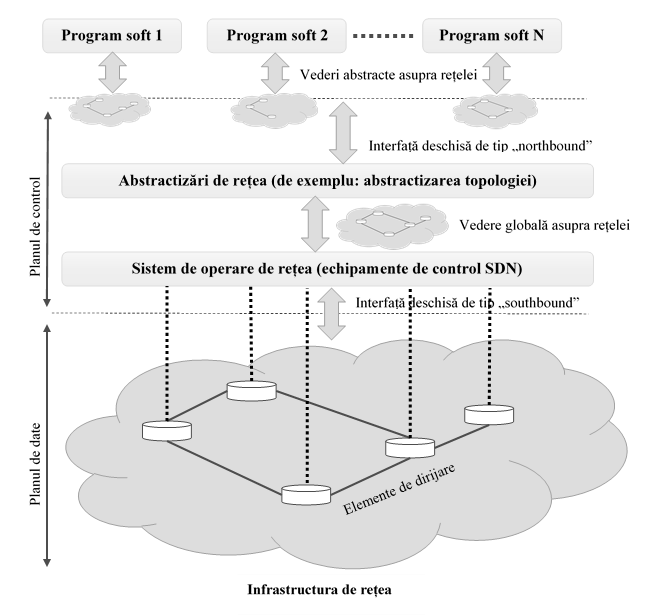
\includegraphics[width=1\textwidth]{arhitectura_sdn}
	\caption{Arhitectura SDN și abstractizările fundamentale~\cite{kreutz2015software}}
	\label{fig:arhitectura_sdn}
\end{figure}

În mod ideal, \textit{abstractizarea dirijării} reprezintă permiterea oricărui comportament de dirijare dorit de aplicațiile software din rețea (cu ajutorul planului de control),  fără a necesita cunoașterea detaliilor legate de capabilitățile hardware ale infrastructurii existente. Un exemplu pentru o astfel de abstractizare este protocolul OpenFlow.

\textit{Abstractizarea distribuției} se referă la faptul că aplicațiile \gls{sdn} nu ar trebui să cunoască problemele stărilor distribuite din rețea, transformând problemele unui plan de control distribuit, cum era în rețelele tradiționale, într-un plan de control logic centralizat. Acesta este realizat printr-un nivel comun de distribuţie, în \gls{sdn} fiind reprezentat de sistemul de operare de rețea. Acesta are două mari funcții: instalarea comenzilor de control pe echipamentele de dirijare și colectarea de informaţii despre starea planului de date, pentru a putea oferi programelor software o vedere de ansamblu asupra rețelei.

\textit{Abstractizarea specificărilor} reprezintă capabilitatea unui program software din rețea de a exprima un anume comportament al acesteia fără a fi responsabil personal și de implementarea acestui comportament. Acest lucru se poate realiza prin soluții de virtualizare, precum și cu ajutorul limbajelor de programare de rețea.

Arhitectura \gls{sdn} poate fi privită ca o structură cu mai multe niveluri, având fiecare funcțiile sale specifice. Unele niveluri sunt necesare în orice implementare \gls{sdn}, în timp ce altele pot fi prezente doar în anumite implementări particulare. Aceste niveluri sunt ilustrate în Figura \ref{fig:niveluri_sdn} și vor fi prezentate în continuare \cite{kreutz2015software}.

\begin{figure}[h]
	\centering
	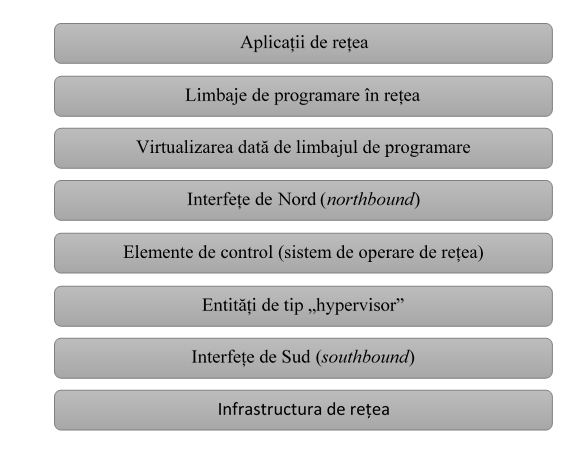
\includegraphics[width=1\textwidth]{niveluri_sdn}
	\caption{Nivelurile rețelelor definite prin software}
	\label{fig:niveluri_sdn}
\end{figure}


\paragraph{Nivelul 1: Infrastructura}

Infrastructura pentru o rețea definită prin programe software este compusă, la fel ca în cazul rețelelor tradiționale, din echipamente de rețea (comutatoare, rutere, echipamente de transport de date etc.). Însă, diferenţa majoră constă în faptul că, în \gls{sdn}, echipamentele de rețea sunt simple elemente de dirijare de trafic, inteligenţa lor fiind mutată în echipamentele de control \gls{sdn} și în aplicațiile software. O altă diferenţă importantă este aceea că echipamentele care constituie infrastructura de rețea trebuie să implementeze interfețe standard (cum ar fi OpenFlow), care să asigure compatibilitatea comunicației și a configurărilor, dar și interoperabilitatea cu alte echipamente, atât din planul de control cât și din cel de date, indiferent de producător. Acest lucru era destul de dificil în rețelele tradiționale, din cauza multitudinii de interfețe proprietare.

În paradigma \gls{sdn}, elementele care alcătuiesc infrastructura rețelei nu mai iau deciziile de dirijare pe baza adresei destinație, ca în cazul rețelelor tradiționale, ci pe baza unor fluxuri de date \cite{mckeown2008openflow}. Presupunând o rețea bazată pe protocolul OpenFlow, elementele de dirijare se bazează pe o secvenţă de tabele de fluxuri, unde fiecare intrare din tabel conţine: (i) o regulă de asociere, (ii) acțiunile care trebuie executate asupra pachetelor care se potrivesc regulii și (iii) contoare care să menţină o statistică despre pachetele care s-au potrivit. Prioritatea regulilor este dată de ordinea din tabelul de fluxuri. Acțiunile posibile asupra pachetelor pot fi: dirijarea acestora către un port de ieșire, dirijarea către echipamentul de control, aruncarea pachetelor, trimiterea către secvența normală de prelucrare, trimiterea către următorul tabel de fluxuri etc. Regulile de potrivire care se pot aplica pachetelor se pot baza pe mai multe câmpuri din antetul pachetului, cum ar fi câmpuri de nivel doi (Ethernet), MPLS, de nivel 3 (IPv4/v6), câmpuri de nivel 4 (TCP/IP) etc., în aproape orice fel de combinație.

\paragraph{Nivelul 2: Interfețele de Sud (\textit{southbound})}

Interfețele de Sud fac legătura între echipamentele de dirijare și echipamentele de control din rețea, îndeplinind astfel una dintre funcțiile de bază ale rețelelor definite prin programe soft: separarea planurilor de date și de control. Terminologia Nord/Sud se raportează la controlerul \gls{sdn}.

Acest tip de interfețe este foarte bine privit de către industrie. Prin standardizarea acestora se va permite construirea de rețele cu echipamente care să poată proveni de la mai multi producători, promovând astfel interoperabilitatea.

Cel mai acceptat și utilizat standard pentru acest tip de interfețe este OpenFlow. Acesta propune specificaţii comune pentru implementarea canalului de comunicaţie dintre echipamentele de dirijare și cele de control. Protocolul OpenFlow furnizează trei surse de informații pentru sistemul de operare de rețea: (i) mesaje bazate pe evenimente, care sunt trimise de echipamentele de dirijare către cele de control în momentul în care apare o schimbare a legăturii de date sau a unui port; (ii) statistici despre fluxurile de date, care sunt generate în echipamentele de dirijare și trimise către echipamentele de control; (iii) mesaje care conţin și pachete de date și sunt trimise de către echipamentele de dirijare către cele de control în momentul în care nu ştiu cum să trateze un anumit tip de flux de date sau din cauza faptului că există o acțiune explicită de tipul \textit{trimite la echipamentul de control} în tabela de fluxuri. Aceste tipuri de informații sunt esențiale pentru furnizarea de detalii despre fluxurile de date sistemului de operare de rețea.

Deşi este cel mai utilizat protocol, OpenFlow nu este singura interfață de Sud pentru rețelele definite prin programe soft. Există și alte propuneri pentru acest tip de interfețe, dintre care amintim: \gls{netconf}, \gls{forces}, OpFlex, \gls{pof}, \gls{ovsdb}, \gls{rofl}, \gls{hal}, OpenState etc. \cite{haleplidis2015network, zhou2014research, onfts016}.

\paragraph{Nivelul 3: Entitățile de tip \textit{hypervisor} de rețea}

Entităţile de tip \textit{hypervisor} reprezintă o soluție software, firmware, sau hardware care creează și rulează mașini virtuale. Acestea permit unor mașini virtuale distincte să partajeze aceleași resurse hardware. Astfel au apărut noi modele de afaceri și tehnologii, cum ar fi aplicațiile de tip cloud, unde fiecare utilizator poate avea resursele sale virtuale, de la puterea de calcul până la spaţiul de stocare. Din păcate, acest model nu a putut fi aplicat și pentru resursele de rețea, acestea fiind configurate în continuare în mod static și independent una față de cealaltă.

Există două cerinţe ale aplicațiilor de la rețea: spaţiul de adresare și topologia rețelei. Volume diferite de muncă necesită diferite servicii și topologii de rețea, însă acestea sunt greu de oferit de către o singură topologie fizică. De asemenea, aplicațiile care rulează într-un mediu virtualizat funcționează în același spațiu de adresare ca infrastructura fizică. Astfel, mașinile virtuale nu pot migra în locuri arbitrare, deoarece schema de adresare este fixă și greu de modificat.

Soluția la această problemă ar fi ca rețeaua să ofere la rândul ei virtualizare, din punctul de vedere al topologiei și al spațiului de adresare. Apoi, fiecare aplicație care rulează într-o mașină virtuală ar avea posibilitatea să configureze atât nodurile de calcul cât și rețeaua, în același timp. Acest lucru nu este posibil prin tehnologiile actuale, cum ar fi \gls{vlan} - domeniu virtualizat de nivel 2, \gls{nat} - spațiu de adresare IP virtualizat și \gls{mpls} - rute virtuale, deoarece rețeaua nu se poate reconfigura într-un mod global, fiind nevoie ca fiecare element de rețea să fie reconfigurat individual \cite{kreutz2015software, peng2012vdn, koponen2014network}.

Rețelele definite prin software încearcă să ofere posibilitatea de virtualizare a rețelei, prin această entitate de tip \textit{hypervisor}. Există mai multe propuneri în acest sens, dintre care amintim: FlowVisor, \gls{nvp}, FlowN, RadioVisor, IBM SDN VE, OpenVirteX, HyperFlex, \gls{xdpd} etc. \cite{sherwood2009flowvisor, gudipati2014radiovisor, al2014openvirtex, sune2013xdpd, blenk2015hyperflex}.

\paragraph{Nivelul 4: Echipamentele de control / Sistemul de operare de rețea}

Sistemele de operare tradiționale oferă abstractizări pentru accesarea resurselor hardware, pentru administrarea accesului concurent la resurse și pentru a oferi mecanisme de securitate și protecție. Prin contrast, rețelele au fost administrate și configurate până acum cu ajutorul unor instrucțiuni de nivel jos, specifice fiecărui echipament și cu sisteme de operare de rețea proprietare (cum ar fi IOS de la Cisco sau JunOS de la Juniper). Acestea nu furnizează abstractizări care să ofere, într-un mod transparent, funcționalități de bază \cite{kreutz2015software}.

În cadrul \gls{sdn} se încearcă găsirea unor soluții în acest sens, printr-un control logic centralizat, oferit de un sistem de operare de rețea. Acesta va trebui să ofere abstractizări, care să fie apoi folosite de dezvoltatorii de aplicații software. Printre serviciile oferite de sistemul de operare de rețea ar trebui să se regăsească funcționalități generale, cum ar fi: descoperirea dispozitivelor de rețea, distribuirea configuraţiei rețelei, starea rețelei sau informații despre topologia rețelei.

Echipamentul de control este elementul critic din arhitectura \gls{sdn}, deoarece el va trebui să interpreteze aplicațiile dezvoltate pentru administrarea rețelei și să genereze configurația acesteia pe baza politicilor definite acolo. Există deja o multitudine de echipamente de control propuse pentru a fi utilizate în arhitectura \gls{sdn}, diferite în foarte multe aspecte. Unul dintre cele mai importante, care diferențiază echipamentele de control, este tipul arhitectural folosit: centralizat sau distribuit \cite{dixit2013towards, levin2012logically, jimenez2014controller}.

Un echipament de control centralizat reprezintă o entitate care administrează toate dispozitivele din planul de date al rețelei \cite{ome2012software}. În mod natural, acesta poate fi privit ca un punct unic de defectare a rețelei și ar putea aduce limitări în extensibilitatea acesteia, deoarece este posibil ca un singur echipament de control să nu fie suficient pentru administrarea unui număr mare de echipamente de dirijare. Printre propunerile de astfel de echipamente de control se numără: Maestro, Beacon (care poate administra un număr foarte mare de fluxuri de date, undeva la 12 milioane de fluxuri pe secundă, conform~\cite{erickson2013beacon}), NOX-MT, sau Floodlight. Acestea se bazează pe mai multe fire de execuție și pe paralelismul oferit de arhitecturile de calculatoare cu mai multe nuclee.

Pe de altă parte, un sistem de operare de rețea distribuit poate rezolva problema extensibilităţii rețelei, fiind potrivit pentru orice tip de rețea. Această distribuţie poate fi realizată printr-un grup de echipamente de control care să se afle în același loc, sau printr-un set de dispozitive distribuite fizic în mai multe locuri. Această ultimă variantă ar putea fi mai potrivită pentru prevenirea diferitelor defecţiuni logice sau fizice. Câteva exemple de astfel de echipamente de control distribuite: Onix \cite{koponen2010onix}, HP VAN SDN, PANE, HyperFlow \cite{tootoonchian2010hyperflow}, \gls{onos}~\cite{berde2014onos} sau \gls{odl}~\cite{medved2014opendaylight}, SMaRtLight \cite{botelho2014smartlight} etc.

Însă, în cazul echipamentelor de control distribuite, apare o problemă destul de importantă: consistenţa datelor. Toate echipamentele de control ar trebui să citească aceeaşi valoare imediat după ce aceasta a fost scrisă, pentru a evita cazul când dispozitivele de control au imagini diferite asupra rețelei. Majoritatea propunerilor de până acum oferă doar o \textit{consistență scăzută}, ceea ce înseamnă că, după ce o valoare a fost scrisă într-un nod de control, valoarea se va reflecta, \textit{la un moment dat}, în toate nodurile de control. Acest lucru implică o perioadă de timp în care dispozitivele de control au viziuni diferite asupra rețelei. Există și propuneri de echipamente de control care oferă o \textit{consistență ridicată} (Onix și SMaRtLight) \cite{koponen2010onix, botelho2014smartlight}, care garantează citirea aceleiaşi valori de către orice nod de control, imediat după scrierea acesteia.

Există și situaţii unde o abordare hibridă ar fi cea mai potrivită, o arhitectură în care să existe grupuri de echipamente de control într-o parte de rețea și dispozitive de control distribuite în alte locuri din rețea.

\paragraph{Nivelul 5: Interfețe de Nord (\textit{northbound})}

Interfețele de Nord, împreună cu cele de Sud constituie cele mai importante două abstractizări din arhitectura rețelelor definite prin software. Dacă cele din urmă asigură comunicaţia dintre echipamentele de control și dispozitivele din planul de date al rețelei, fiind astfel mai mult orientate spre hardware, interfeţele de Nord alcătuiesc, în mare parte, un ecosistem software. Încă nu există un astfel de tip de interfețe care să fie acceptat la scară largă, cum este OpenFlow în cazul celor de Sud, însă acest lucru se va întâmpla probabil, pe măsură ce paradigma \gls{sdn} se va maturiza și cazurile de utilizare ale acestui tip de arhitectură de rețea se vor contura mai exact.

Este nevoie ca acest tip de interfețe să fie deschise și standardizate, astfel încât să se asigure interoperabilitatea și portabilitatea programelor soft pe mai multe tipuri de dispozitive de control. Un exemplu în acest sens îl constituie NOSIX~\cite{wundsam2012nosix}. Aceasta este o propunere, care poate fi comparată cu standardul \gls{posix} din sistemele de operare și care oferă abstractizări ce garantează independenţa față de limbajul de programare și dispozitivul de control folosite \cite{barney2009posix}. Dintre celelalte propuneri de interfețe de Nord amintim: RESTCONF, SFNet, Pyretic, NetCore, Frenetic, Nettle etc. \cite{bierman2017restconf, yap2010towards, reich2013modular, monsanto2012compiler}.

\paragraph{Nivelul 6: Virtualizarea dată de limbajul de programare}

Există două caracteristici principale ale soluţiilor de virtualizare date de limbajele de programare: permiterea mai multor niveluri de abstractizare, concomitent cu oferirea proprietăţilor dorite, cum ar fi protecţia și abilitatea de a exprima modularitatea.

Metodele de virtualizare pot permite, de exemplu, diferite imagini asupra unei singure infrastructuri fizice de rețea. Un \textit{comutator virtual} ar putea reprezenta o combinație de mai multe dispozitive de dirijare. Acest mod de lucru simplifică sarcinile dezvoltatorilor de aplicații, care nu trebuie să ţină cont individual de elementele de rețea care alcătuiesc acel \textit{comutator virtual}. Dezvoltarea și implementarea unor aplicații de rețea complexe este simplificată cu ajutorul acestor abstractizări.

O altă formă de virtualizare dată de limbajul de programare o reprezintă împărţirea statică a rețelei în secţiuni. Acest lucru se face de către compilator, bazat pe definiţiile date de nivelul aplicație. După compilare va rezulta un program unitar de control, care are deja implementate funcțiile pentru împărțirea rețelei în bucăţi și comenzile de configurare a acestora. În acest caz nu mai este nevoie de entitatea \textit{hypervisor} care să administreze dinamic bucăţile de rețea.

Există diverse propuneri pentru astfel de soluții de virtualizare, cum ar fi: Pyretic, Splendid, libNetVirt, FlowVisor, IBM SDN VE etc. \cite{reich2013modular, schlesinger2012splendid, turull2012libnetvirt, sherwood2009flowvisor}.

\paragraph{Nivelul 7: limbaje de programare în rețea}

Limbajele de programare au evoluat de la limbaje mașină, specifice hardware-ului, cum era limbajul de asamblare pentru arhitecturile x86, până la limbaje de nivel înalt, cum ar fi Java sau Python. În același mod, limbajele de programare folosite în programarea rețelelor evoluează de la OpenFlow (echivalentul limbajului de asamblare) la limbaje de nivel înalt, cum ar fi Pyretic, Procera, NetCore, Frenetic etc. \cite{reich2013modular, voellmy2012procera, monsanto2012compiler}.

Aceste limbaje de programare de nivel înalt oferă câteva avantaje în contextul rețelelor definite prin software: facilitează dezvoltarea virtualizării rețelei, creează abstractizări care simplifică programarea elementelor de dirijare, promovează modularizarea software și reutilizarea codului în planul de control și chiar îmbunătăţesc dezvoltarea și inovația prin crearea unor medii de lucru mai productive.

Există două tipuri de paradigme de programare în contextul \gls{sdn}: cea declarativă, care este cea mai răspândită și cea imperativă, care este reprezentată doar prin limbajul Pyretic. Paradigma declarativă reprezintă o abordare în care rețelei i se spune ce tip de comportament să aibă și aceasta se va configura (luând singură decizii) astfel încât să îndeplinească acea cerinţă. Paradigma imperativă se referă la situația în care programatorul îi spune rețelei cum să acţioneze și rezultatul va fi cel așteptat, fără ca aceasta să ia propriile decizii.

Scopul \gls{sdn} este ca, în final, să ofere facilități de administrare a rețelelor pe baza infrastructurii definite anterior. Cu ajutorul progreselor din domeniul limbajelor de programare de nivel înalt se va facilita crearea unui ecosistem propice pentru dezvoltarea aplicațiilor \gls{sdn}.

\paragraph{Nivelul 8: Aplicațiile de rețea}

Aplicațiile software vor reprezenta cea mai importantă parte a rețelelor definite prin software, deoarece acestea vor implementa logica de control, care va fi translatată în comenzi ce vor fi instalate la nivelul dispozitivelor din planul de date.

Majoritatea aplicațiilor software din cadrul \gls{sdn} se încadrează într-una din următoarele cinci categorii, conform~\cite{kreutz2015software}: ingineria traficului, securitate și fiabilitate, măsurători și monitorizare, reţelistica centrelor de date, mobilitate și rețele fără fir.

Programele software din categoria mobilitate și microunde își propun să faciliteze implementarea și administrarea rețelelor fără fir, cum ar fi rețelele locale fără fir - \gls{wlan} sau rețelele de telefonie mobilă. Un plan de control distribuit, cum există în momentul de față în rețelele fără fir, nu este optim pentru implementarea mecanismelor de transfer dintre celule, pentru micșorarea interferențelor, pentru alocarea resurselor radio, pentru administrarea spectrului limitat de frecvenţe etc. Aceste probleme sunt adresate în \gls{sdn} și se pot rezolva mai uşor cu ajutorul acestei noi paradigme.

\section{Standardizarea SDN}

Activitățile de cercetare și standardizare din jurul \gls{sdn} au loc pe două planuri importante. Pe de o parte, există organizaţiile care dezvoltă standarde - \gls{sdo}, care sunt formate din reprezentanţi ai industriei, ai academiei, sau alte entități și au ca scop dezvoltarea de specificaţii sau recomandări tehnice, în contextul \gls{sdn} care să fie folosite de toată industria rețelisticii. Autorii din~\cite{schneider2014standardizations} amintesc astfel de organizații: \gls{onf}, \gls{ietf}, \gls{etsi}, \gls{itu-t}, \gls{ieee}. 

Pe de altă parte, există asociații sau comunități de oameni, în general care fac parte din industrie, ale căror rezultate ale cercetării candidează pentru a deveni standarde. Aceste rezultate sunt, de obicei, implementări cu sursă deschisă ce vor fi folosite ulterior în industrie. Exemple de astfel de comunități sunt prezente în~\cite{halpern2014standards, meyer2013software}: OpenDaylight (activităţi ce se desfăşoară sub patronajul fundaţiei Linux), \gls{mef}, \gls{bbf}, \gls{oif}.

Activitățile de standardizare ale \gls{sdn} sunt foarte importante, asigurându-i acestei tehnologii o evoluţie stabilă și aducând-o la o maturitate care îi va permite adoptarea pe scară largă în industria rețelisticii, mitigând astfel dezavantajele rețelelor tradiționale.

Sunt mai multe planuri pe care se lucrează pentru standardizarea \gls{sdn}. Unul dintre aceste planuri este cel al interfeţelor de Sud, care fac legătura între echipamentele de dirijare și echipamentele de control \gls{sdn}. Protocolul OpenFlow este un exemplu în acest sens, însă nu este singurul protocol capabil să facă legătura între planurile de date și de control. În ultimul timp se pune foarte mare accent pe \gls{netconf} ca o alternativă pentru a configura echipamentele care dirijează traficul, după cum se poate observa în~\cite{csoma2015escape, felix2014multi, zhou2014research}. Astfel apare nevoia de a dezvolta modele informaţionale care să abstractizeze echipamentele din planul de date și care să poată fi folosite de \gls{netconf} pentru a configura dispozitivele. Și planul interfeţelor de Nord are un rol important în standardizare, deoarece poate oferi un punct de plecare comun pentru dezvoltatorii de aplicații \gls{sdn}. De exemplu, în cadrul \gls{onf} există un grup care se ocupă cu activităţi de standardizare în această direcţie. Un alt plan este reprezentat de implementările software, cu sursă deschisă (\textit{open-source}), care se crează în acest context. Așa cum evidenţiază și autorii din~\cite{lin2014software, rothenberg2014open}, aceste implementări sunt foarte importante prin ecosistemele care apar ca urmare a activităţii comunităţilor care dezvoltă software cu sursă deschisă.

O importanţă foarte mare în cadrul acestor activităţi o au și demonstraţiile de concept. Acestea au capacitatea de a demonstra avantajele pe care \gls{sdn} le aduce nu doar la un nivel teoretic, ci într-un mod practic, propunând diferite cazuri reale de utilizare a acestei tehnologii și aplicând-o, într-un mod restrâns, unor topologii formate din echipamente reale. Scopul acestora este, pe de o parte, de a adăuga un plus de valoare activităţilor de standardizare și de a testa și proba rezultatele acestor activităţi. Pe de altă parte, aceste demonstraţii de concept au scopul de a atrage atenţia și altor entități din industrie și a duce la înlesnirea adoptării acestei tehnologii pe scară largă.

\subsection{Open Networking Foundation}

\gls{onf} este o organizaţie non-profit formată din peste două sute de membri care fac parte din industrie, academie, sau institute de cercetare, ce are ca obiectiv accelerarea adoptării \gls{sdn} pe scară largă in industria rețelisticii prin dezvoltarea de standarde deschise și de ecosisteme software cu sursă deschisă. \gls{onf} a apărut ca urmare a activităţii de cercetare din jurul protocolului OpenFlow din cadrul Universităţii Stanford. Dintre membrii cei mai importanţi amintim operatori de rețele, precum AT\&T, Google, Facebook, Verizon, Deutsche Telekom sau Telefonica, producători de echipamente, cum ar fi Cisco, Ericsson, Huawei, Intel sau NEC și reprezentanţi ai unor universităţi cunoscute, ca Stanford sau Princeton.

Activitățile din cadrul \gls{onf} sunt împărţite în mai multe zone de interes, conform \cite{onftech}:
\begin{itemize}
	\item \textit{Operatori}. Această zonă se ocupă de mai multe aspecte, precum \gls{sdn} în contextul sistemelor de tip Purtător - \textit{Carrier Grade} - (rețelele de telecomunicaţii foarte sigure, cu o disponibilitate de peste 99,999\% și recuperare în caz de defectare de sub 50 de milisecunde), în centre de date, în întreprinderi sau aspecte legate de migrarea serviciilor dintr-o rețea tradiţională într-o rețea definită prin software.
	\item \textit{Servicii}. Se ocupă de proiecte care permit existența aplicațiilor și serviciilor de rețea care au la bază tehnologia \gls{sdn}. Astfel, există mai multe grupuri de lucru care analizează arhitectura \gls{sdn} și modul în care aceste principii se aplică în imaginea de ansamblu a unei rețele de comunicaţii, un model informaţional \textit{de bază}, care să reprezinte piatra de temelie cu ajutorul căreia să se dezvolte alte modele informaţionale, specializate pentru anumite aplicații sau tehnologii, interfeţele de Nord, pentru a facilita dezvoltarea aplicațiilor \gls{sdn}, probleme de securitate pe care această nouă tehnologie le poate întâmpina.  
	\item \textit{Specificaţii}. Zonă care are ca responsabilitate publicarea tuturor specificaţiilor și recomandărilor tehnice create de \gls{onf}. Acestea includ protocoalele OpenFlow, OF-Config dar și alte interfețe standard care se dezvoltă pentru tehnologii de transport de diferite tipuri (optic, fără fir). Există și un proiect care se ocupă de testare și interoperabilitate, scopul acestuia fiind accelerarea adoptării protocolului OpenFlow prin certificări și promovarea interoperabilităţii între diferiţi producători de echipamente \cite{onftr539}.
	\item \textit{Piaţă}. Această zonă se concentrează pe educarea comunităţii \gls{sdn} în legătură cu valoarea pe care standardele \gls{onf} le oferă rețelelor definite prin software și promovarea adoptării unor astfel de rețele definite prin software cu sursă deschisă. Aceste obiective sunt îndeplinite prin publicaţii, evenimente care se organizează sau demonstraţii care să arate comunităţii cazuri reale de utilizare.
\end{itemize}

Există trei tipuri de publicaţii care reies din activitățile \gls{onf}: (i) \textit{specificaţii}, care includ toate standardele care definesc un protocol, modelul informaţional, funcționalități și documente despre cadrele asociate; publicaţiile normative astfel rezultate se numesc Specificaţii Tehnice - \gls{ts} și sunt supuse unor procese de licenţiere; (ii) \textit{recomandări}, care includ consideraţii arhitecturale, cazuri de utilizare, analiza cerințelor, terminologie; aceste documente referă documente normative \gls{onf}, dar nu necesită licenţiere și pot fi utilizate în mod liber, având rolul de Recomandări Tehnice - \gls{tr}; (iii) \textit{publicaţii}, reprezentând documente care conţin informații ce ajută în procesele de lansare a \gls{sdn} în producție, rezumate ale soluţiilor, studii de caz sau cărţi albe (\textit{white papers}); aceste documente nu au caracter normativ și pot fi folosite în mod liber.

În continuare vor fi enumerate câteva astfel de documente produse de către \gls{onf}: \textit{OpenFlow Switch Specification Ver. 1.5.1} (TS-025), care descrie cerinţele unui comutator logic ce suportă protocolul OpenFlow; \textit{OpenFlow Management and	Configuration Protocol 1.2 (OF-Config 1.2)} (TS-016), document ce descrie motivația, cerințele, scopul și specificaţiile protocolului OF-Config; \textit{Conformance Test Specification for OpenFlow Switch Specification V1.3.4} (TS-026), definind cerinţele și procedurile de test care determină conformitatea unui comutator cu specificațiile protocolului OpenFlow 1.3.4; \textit{Core Information Model (CoreModel) 1.2} (TR-512), care prezintă modelul informațional de bază, pe care celelalte modele informaționale dezvoltate în \gls{onf} se bazează; \textit{Microwave Information Model} (TR-532), reprezentând modelul informațional ce descrie echipamentele de transport de date fără fir. Aceste ultime două documente vor fi detaliate în următorul capitol, fiind baza dezvoltării și implementării simulatoarelor propuse în această lucrare.

Un rol important în adoptarea \gls{sdn} de către operatori și în diseminarea rezultatelor din cadrul \gls{onf} îl au demonstraţiile de concept. Acestea adună laolaltă operatori, producători de echipamente și integratori de servicii, cu scopul de a demonstra recomandările produse de activitatea de cercetare. În contextul rețelelor de transport de date fără fir, proiectul \gls{wt}, care face parte din grupul \gls{otwg}, a terminat cu succes patru astfel de demonstraţii de concept~\cite{onf2015_poc1, onf2016_poc2, onf2016_poc3, onf2017_poc4}.

Prima astfel de demonstraţie a avut loc în octombrie 2015, în Madrid și a fost organizată de Telefonica, împreună cu Universitatea Carlos III. Scopul acesteia a fost de a extinde protocolul OpenFlow cu atribute specifice echipamentelor de transport de date fără fir. Astfel, interfaţa de Sud folosită a fost OpenFlow, în timp ce echipamentul de control \gls{sdn} a fost \gls{onos}. Au fost prezentate două cazuri de utilizare: (i) pornirea/oprirea unei interfeţe radio în funcţie de nivelul de trafic ce trebuie transmis de către echipament, economisind astfel energie în momentele în care nivelul de trafic în reţea nu este foarte ridicat; (ii) schimbarea căilor de date într-un ruter, în cazul în care se pierd pachete pe legătura radio, ca urmare a unor schimbări meteorologice (simulate prin folosirea unui atenuator variabil pe legătura radio).

A doua demonstraţie de concept a avut loc în aprilie 2016, la München și a fost organizată de Telefonica. Spre deosebire de prima demonstraţie, în cea de-a doua s-a folosit drept interfaţă de Sud protocolul \gls{netconf}, iar echipamentul de control \gls{sdn} a fost \gls{odl}. Ca model informaţional YANG pentru configurarea echipamentelor s-a ales un model pentru microunde simplificat (conţinea un număr limitat de atribute). Acesta a fost dezvoltat de către grup și apoi implementat de către echipamentele de la diferiţi producători. Au fost demonstrate mai multe cazuri de utilizare folosind aplicaţii \gls{sdn} care se bazează pe acel model: detectarea și configurarea de noi echipamente, detectarea și corecţia (printr-o acţiune a operatorului) diferenţelor între configuraţia curentă și cea planificata, detecţia și vizualizarea reţelei de transport configurate, primirea, afişarea și stocarea evenimentelor și alarmelor din reţea.

Cea de-a treia demonstraţie de concept s-a desfăşurat în octombrie 2016 și a avut loc în centrul de cercetare WINLAB de la Universitatea Rutgers, fiind organizat de AT\&T. S-au ales aceeaşi interfaţă de Sud și acelaşi echipament de control \gls{sdn}, scopul acestei demonstraţii fiind de a proba utilitatea întregului model informaţional pentru microunde (conţinea toate atributele pe care le poate avea un echipament de transport de date fără fir). S-a implementat și modelul de bază (\textit{Core Model}), dezvoltat de alt grup din cadrul \gls{onf}. Au fost demonstrate aplicaţiile dezvoltate pentru cea de-a doua demonstraţie, dar și două noi aplicaţii: una care administrează spectrul, prin compararea și configurarea frecvenţelor planificate și cele configurate pe echipamente, realocându-le în caz că nu se potrivesc; cealaltă, denumită automatizarea în bucla închisă, demonstra un răspuns simplist la anumiţi factori declanşatori (interni, externi sau temporali).

A patra demonstraţie de concept a avut loc în iunie 2017, la Bonn și a fost organizată de Deutsche Telekom. S-au folosit mai multe modele informaţionale: modelul pentru microunde, modelul de bază, un model Ethernet simplificat și un model pentru sincronizare - pentru \gls{ptp}, plecând de la un model dezvoltat de ITU-T. Astfel, s-au putut demonstra mai multe cazuri de utilizare: administrarea echipamentelor care transportă date fără fir, administrarea indicatorilor de performanță ai echipamentelor, administrarea puterii echipamentelor, administrarea echipamentelor capabile Ethernet, recalcularea căilor de trafic Ethernet într-o rețea sau administrarea echipamentelor care suportă \gls{ptp}. 

\subsection{IETF}

Un alt \gls{sdo} care prestează activităţi de standardizare în domeniul rețelelor definite prin software este \gls{ietf}. Această organizaţie, în general, oferă standardele de bază folosite în Internet. Obiectivul lor declarat este îmbunătăţirea funcţionării Internetului prin dezvoltarea de documente tehnice relevante și de înaltă calitate care să ghideze proiectarea, utilizarea și administrarea Internetului.

Doar puține din grupurile de lucru din cadrul \gls{ietf} se ocupă cu activităţi care au legătură cu tehnologia \gls{sdn}. Unul dintre acestea a dezvoltat \gls{forces}, iniţiativă ce separa planurile de date și de control ale echipamentelor \cite{doria2010forwarding}, cu câțiva ani înainte ca protocolul OpenFlow, mult mai cunoscut, să propună asta într-un mod care să permită o adoptare mai rapidă în industrie.

Alt grup de lucru se ocupă de \textit{interfaţa către sistemul de rutare} - \gls{i2rs}. Acesta își propune să dezvolte interfețe pentru ca aplicațiile \gls{sdn} să poată accesa sistemul de rutare al rețelei. Se doreşte ca beneficiarii \gls{i2rs} să fie aplicații de administrare, echipamente de control \gls{sdn} sau aplicații de utilizator care au cereri specifice la adresa rețelei. Acestea ar permite informaţiilor, politicilor și parametrilor operaţionali să fie introduşi sau extraşi din sistemul de rutare, fără a afecta consistenţa datelor și coerenţa infrastructurii de rutare. Această abordare poate fi privită ca un rival al protocolului OpenFlow, cu menţiunea că se aplică doar de la nivelul 3 în sus, în stiva OSI.

În interiorul grupului de lucru \gls{spring} se discută un control al rutării care să permită indicarea unei căi de dirijare încă de la sursa de trafic \cite{schneider2014standardizations}, calcularea acesteia putând fi făcută atât centralizat, cât și distribuit. Tot în cadrul \gls{ietf} se dezvoltă și protocolul \gls{netconf}, însă acesta va fi detaliat într-o secţiune viitoare.

Parte din \gls{ietf} este și \gls{irtf}. Aceasta este o organizaţie paralelă, care se ocupă mai mult de partea de cercetare, sprijinind proiectele care se crede că vor fi benefice comunităţii Internetului, dar care nu sunt încă pregătite pentru implementare. Aici există un grup de lucru care investighează tehnologia \gls{sdn} din mai multe perspective, cu scopul de a recunoaşte atât abordări ce pot fi definite și lansate pe termen scurt, dar și provocări viitoare: \gls{sdnrg}. Sunt de interes probleme ca extensibilitatea soluţiei, abstractizări sau limbaje de programare ce pot fi folosite în contextul \gls{sdn}. Se doreşte ca acest grup să ofere un spațiu comun tuturor cercetătorilor cu interes în acest domeniu.

%\subsection{ETSI}
%
%Unul dintre grupurile specificaţiilor pentru industrie din cadrul \gls{etsi} se numeşte grupul \gls{nfv}. Conceptul de virtualizare a funcţiilor de rețea este unul complementar rețelelor definite prin software. Este o iniţiativă a operatorilor de rețea și are ca scop să permită acestora să profite de noile tehnologii ce apar, să le crească abilităţile de a livra servicii, să reducă costurile și să crească viteza de lansare în producție a serviciilor noi sau experimentale.
%
%Chiar dacă accentul este pus pe virtualizarea funcţiilor de rețea, a fost foarte bine înţeles faptul că utilizarea tehnologiei \gls{sdn} reprezintă un avantaj major și că multe dintre cazurile de utilizare propuse pot fi implementate folosind această paradigmă. Astfel, grupul lucrează la standardizare și stabileşte protocoale împreună cu celelalte organizaţii care se ocupă de standardizarea \gls{sdn}.
%
%\subsection{ITU-T}
%
%Unul dintre cele mai vechi organizaţii de standardizare, \gls{itu-t}, a avut o importanţă majoră în multe aspecte critice din domeniul telecomunicaţiilor. În contextul \gls{sdn}, grupul se ocupă de în principal de arhitectura și cerinţe pentru utilizarea acestei tehnologii în rețelele de transport de date. Deoarece acest tip de rețele au cerinţe importante, diferite de celelalte rețele, evidenţierea acestora de către \gls{itu-t} ajută la orientarea eforturilor de standardizare în direcţia corectă. 
%
%Zonele de interes pentru grupurile care fac parte din această organizaţie sunt: aspecte arhitecturale ale securităţii în \gls{sdn} și servicii pentru securitate prin \gls{sdn}, specificaţii pentru arhitectura planului de control în rețele de transport de date, cerinţe de semnalizare folosind tehnologia \gls{sdn} sau cerinţe funcţionale și arhitecturale pentru \gls{sdn} și rețelele viitorului.

\section{SDN în contextul reţelelor actuale}

Chiar dacă nu este o tehnologie ajunsă la maturitate în toate aspectele unei rețele, paradigma \gls{sdn} este deja folosită în rețele de producție de anumite tipuri. Autorii din \cite{alvizu2017comprehensive} evidenţiază faptul că evoluția \gls{sdn} este susţinută de către trei mari porţiuni ale industriei rețelisticii: furnizorii serviciilor de tip \textit{cloud} (care utilizează mari centre de date), furnizorii de servicii de telecomunicaţii și întreprinderile, așa cum se poate observa și în Figura \ref{fig:sdn_network_deployments}. 

\begin{figure}[h]
	\centering
	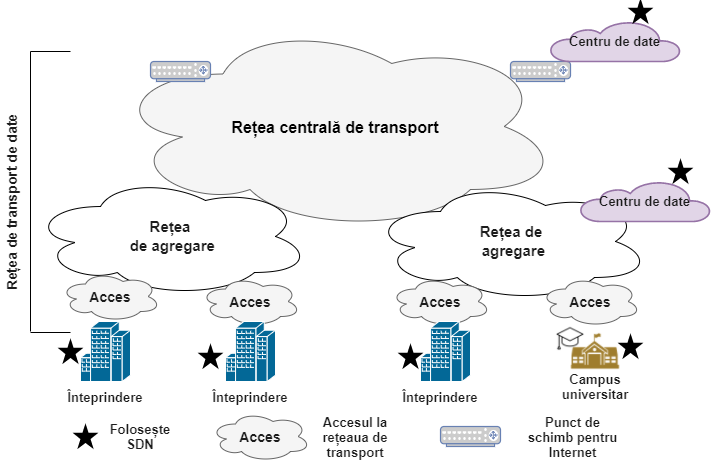
\includegraphics[width=1\textwidth]{sdn_network_deployments}
	\caption{Implementarea SDN în contextul rețelelor actuale~\cite{alvizu2017comprehensive}}
	\label{fig:sdn_network_deployments}
\end{figure}

Astfel, \gls{sdn} este implementat deja cu succes în rețelele unor campusuri universitare (Universitatea Stanford, de exemplu, dat fiind faptul că această paradigmă își are originile acolo), în mari centre de date sau în întreprinderi. În cazul rețelelor de transport, încă se duc activităţi de standardizare care să permită operatorilor rețelelor de telecomunicaţii să implementeze această tehnologie în cel mai scurt timp, beneficiind astfel de avantajele pe care aceasta le oferă (cel mai important, din punctul lor de vedere, fiind reducerea costurilor).

Această secţiune va prezenta în continuare utilizarea \gls{sdn} la momentul actual, în mai multe contexte actuale: în rețelele din marile centre de date, în rețelele de tip hibrid, care combină rețelele tradiționale cu \gls{sdn} sau prin studii de caz, implementări sau experimente efectuate pe teren (în rețele de producție).

\subsection{SDN în centrele de date}

Centrele de date reprezintă grupări de calculatoare cu putere mare de procesare și capacitate mare de stocare. Această idee nu este una nouă, fiind prezentă de câteva decenii, însă în timp au evoluat aceste caracteristici ale calculatoarelor, precum și numărul lor într-un centru de date. În zilele noastre acestea au ajuns sa conţină mii sau chiar zeci de mii de mașini fizice (servere) \cite{goransson2016software}.

Creșterea numărului de servere și a puterii de stocare, combinate cu creșterea vitezei și a lățimii de bandă din rețea a dus la dorința de a stoca din ce în ce mai multă informație în centre de date tot mai mari. În mod natural, acest lucru va însemna combinarea centrelor de date pentru a forma altele mai mari. Pe lângă acest aspect, se pune foarte mare accent în ultimul timp pe tehnologii de virtualizare, care permit unui server rularea mai multor mașini virtuale, pentru diferite aplicații sau servicii ale utilizatorilor.

A fost creat astfel un mediu dinamic, atât în cadrul centrelor de date, cât și între acestea. După cum este prezentat și în \cite{onf_openflow_backbone2012}, operații precum prevenirea sau recuperarea în caz de dezastru, sau balansarea încărcării severelor au nevoie de o creștere a traficului între centrele de date, lucru ce duce la o administrare complexa a acelei rețele.

Centrele de date sunt folosite și în cazul oferirii de servicii de virtualizare de servere. Operaţiunile într-un astfel de mediu implică lucrul cu mașini virtuale și, de cele mai multe ori, necesitatea migrării acestora între diferite mașini sau centre de date. Asta înseamnă că diferite aplicații sau servicii trebuie să aibă o vedere proprie asupra rețelei dintre servere, care este doar o vedere la nivel logic, în comparaţie cu rețeaua fizică existentă. Așa cum este prezentat și în \cite{nadeau2013sdn}, crearea de astfel de rețele logice se poate face si fără \gls{sdn}, prin metode folosite și în rețelele tradiționale, cum ar fi cu ajutorul unor \gls{vlan}-uri. Însă, în cazul centrelor de date foarte mari, acestea pot fi insuficiente. Cum ele pot fi exprimate într-un pachet Ethernet doar prin 12 biţi, numărul maxim de rețele virtuale este 4096. Apare astfel nevoia unor alte metode, care sunt însă mai complex de configurat.

O metodă pentru crearea de rețele logice care să fie prezentate unor aplicații sau servicii este chiar folosirea tehnologiei \gls{sdn}, făcând abstracţie de rețeaua fizică. În \cite{onf_openflow_backbone2012, onf_sdn_datacenter2013, liu2014sdn, munoz2015integrated} se prezintă diferite metode care pot fi aplicate în astfel de cazuri, sau care chiar au fost demonstrate.

Soluția \gls{sdn} a fost chiar aplicată în rețele de producție. Așa cum se explică în \cite{google_casestudy}, centrele de date ale Google folosesc deja această soluție, cu ajutorul protocolului OpenFlow. Există două laturi ale rețelei de arie largă - \gls{wan} folosită de Google: o parte legată la Internet, care conţine traficul utilizatorilor și o parte internă, care transportă traficul dintre centrele de date. Cele două au caracteristici diferite ale traficului și, implicit, nevoi diferite. În acea rețea internă a fost implementat \gls{sdn}, prin protocolul OpenFlow. Avantajele evidenţiate de Google includ o viziune de ansamblu asupra rețelei, un răspuns mai rapid la erori, timp mai scurt de implementare, actualizări mai rapide ale software-ului rețelei, fără pierdere de trafic sau existența unui mediu de test de mare fidelitate. Chiar dacă în 2012, atunci când a fost implementată această tehnologie în rețea, protocolul OpenFlow era încă la început și nu avea toate facilităţile pe care le oferă astăzi, Google a arătat încă de atunci că tehnologia \gls{sdn} poate fi folosită, aducând foarte multe avantaje, în multe cazuri de utilizare din industria rețelisticii.

\subsection{SDN în rețelele hibride}

Rețelele hibride reprezintă o combinație între rețelele tradiționale și \gls{sdn}, având scopul de a combina avantajele aduse de ambele, cât timp tehnologia \gls{sdn} nu este încă destul de matură și prezintă unele dezavantaje. Un alt motiv pentru apariția acestor rețele hibride este imposibilitatea de a schimba rețelele de producție într-un timp foarte scurt, în același timp asigurând și funcționarea acestora în parametrii agreaţi.

Autorii din \cite{vissicchio2014opportunities} prezintă oportunităţile și provocările aduse de o astfel de abordare. Ei propun patru modele ale rețelelor hibride: (i) rețele hibride bazate pe topologie, (ii) rețele hibride bazate pe servicii, (iii) rețele hibride bazate pe clase și (iv) rețele hibride integrate. Avantajele prezentate de aceste modele hibride sunt flexibilitatea, robusteţea, extensibilitatea, costuri mai mici ale implementării, date de faptul ca nu toată rețeaua este actualizată. Pe de altă parte, această abordare vine și cu dezavantaje, reprezentate de nevoia de a administra paradigme eterogene și garantarea faptului că interacţiunea dintre ele este benefică.

În \cite{hong2016incremental, levin2013toward, canini2016panopticon} se propun sisteme care să permită o implementare incrementală a \gls{sdn} în rețele de tip hibrid pentru rețele ale întreprinderilor și ale furnizorilor de servicii. Autorii evidenţiază faptul că implementarea directă, într-o rețea de producție a acestei noi tehnologii este imposibilă și ar conduce atât la probleme de implementare, cât și la probleme operaționale în rețea. Ei susţin că implementarea \gls{sdn} în puncte cheie ale rețelelor va aduce avantajele acestei tehnologii, fără nevoia de a înlocui toată rețeaua de la început. Pentru a determina aceste puncte cheie, autorii propun un \textit{planificator al implementării}, care să analizeze topologia de rețea, împreună cu informaţiile istorice despre trafic și constrângeri de resurse.

Lucrarea \cite{jin2015telekinesis} prezintă o altă abordare pentru aceste rețele hibride. Autorii propun un echipament de control al rețelei care să poată interacţiona atât cu echipamentele care folosesc un control centralizat, cât și cu cele care au un control distribuit. Controlarea echipamentelor vechi din rețea, care nu suportă protocolul OpenFlow se face chiar cu ajutorul acestuia. Astfel, dacă se vrea alterarea fluxului de date dintr-un echipament vechi, autorii propun folosirea unei extensii a OpenFlow, numită \textit{LegacyFlowMod}, care să instruiască un echipament OpenFlow să trimită un alt pachet special către echipamentul vechi, astfel încât acesta să își schimbe tabela de dirijare.

Autorii din \cite{caria2015divide, caria2016link} susţin de asemenea că o soluție hibridă este mai potrivită. Propun astfel folosirea unor rețele care să combine \gls{sdn} cu protocolul \gls{ospf}, păstrând avantajele date de acest protocol vechi de rutare, care a fost folosit cu succes câteva zeci de ani și, în același timp, aducând și câteva din avantajele propuse de \gls{sdn}.

\subsection{Studii de caz. Implementări. Experimente în rețele de producție}

Există numeroase studii de caz sau experimente în rețele de producție care demonstrează utilitatea \gls{sdn} și faptul că această tehnologie poate fi implementată cu succes în rețelele din zilele noastre.

În \cite{nec2012hospital} se prezintă soluţia implementată în rețeaua spitalului \textit{Kanazawa University}, din Japonia. S-a folosit tehnologia \gls{sdn}, cu ajutorul protocolului OpenFlow pentru a uşura munca de administrare a rețelei spitalului, care devenea din ce în ce mai complexă, pe măsură ce noi echipamente medicale trebuiau adăugate. Rețeaua, fiind operată de personalul spitalului, era vulnerabilă la erorile provocate de greşelile umane. Trebuia asigurată izolarea între anumite departamente ale spitalului, în unele cazuri, astfel că administrarea rețelei devenea greoaie. Cu ajutorul \gls{sdn} a fost creată o soluție în care infrastructura de rețea este uşor de administrat, prin aplicații software care rulează deasupra echipamentului de control \gls{sdn}, permiţând departamentelor crearea de rețele virtuale proprii, asigurând în același timp conectivitate între departamente. Astfel, rețeaua spitalului a devenit stabilă și pregătită pentru dezvoltările rapide care apar în industria medicală în zilele noastre.

Lucrarea \cite{bidkar2014field} ilustrează folosirea \gls{sdn} în cadrul unei rețele optice de transport a unui furnizor de servicii prin Ethernet. Autorii au implementat această tehnologie pentru oferirea de servicii în acea infrastructură de rețea. Obiectivele urmărite au fost simplificarea administrării rețelei și furnizarea de trafic, în funcție de serviciul solicitat (de exemplu, lățime de bandă la cerere).

În \cite{kalman2014applicability} se analizează posibilitatea folosirii tehnologiei \gls{sdn} în rețelele Ethernet industriale. Autorul evidenţiază punctele în care această tehnologie s-ar putea aplica în rețelele industriale și avantajele pe care o astfel de implementare le-ar aduce.

Autorii din \cite{kobayashi2014maturing} urmăresc evoluția implementărilor \gls{sdn} pornind de la nivelul unei rețele dintr-un simplu laborator din cadrul Universităţii Stanford și până la rețele de nivel naţional. Cu ajutorul acestor studii se evidenţiază compromisurile care apar în implementarea acestei noi tehnologii în rețele de producție. De exemplu, pentru o simplă rețea a unui campus universitar, un singur server poate susţine tot planul de control al rețelei, incluzând echipamentul de control și diferitele aplicații care rulează acolo pentru administrarea acesteia. Primele cazuri de utilizare demonstrate cu ajutorul \gls{sdn} au fost rutarea pe cea mai scurtă cale de nivel 2, învăţarea adreselor de nivel 2 - \gls{mac}, descoperirea topologiei cu ajutorul \gls{lldp} sau colectarea de statistici de la comutatoarele din rețea. Aceste experimente au relevat câteva aspecte importante pentru performanţelor rețelelor \gls{sdn}: timpul necesar configurării fluxurilor de date în rețea, numărul de intrări în tabelele de fluxuri ale comutatoarelor. De asemenea, este important ca un comutator să fie hibrid, adică să suporte atât protocolul OpenFlow, cât și pe cele tradiționale. O altă fază a experimentelor conduse de aceşti autori a constat în împărțirea infrastructurii de rețea în mai multe rețele logice destinate diferitor aplicații. 

Toate aceste experimente și studii de caz prezentate au avut la bază protocolul OpenFlow, ducând la evoluția acestuia. Acest lucru nu trebuie să ne ducă însă cu gândul că tehnologia \gls{sdn} înseamnă doar OpenFlow. După cum se va vedea în capitolele următoare, în special în cazul rețelelor de transport de date prin microunde, există și alte protocoale cu ajutorul cărora se pot aduce principiile \gls{sdn} în rețea.

